\documentclass{ximera}

\graphicspath{  
{./}
{./whoAreYou/}
{./drawingWithTheTurtle/}
{./bisectionMethod/}
{./circles/}
{./anglesAndRightTriangles/}
{./lawOfSines/}
{./lawOfCosines/}
{./plotter/}
{./staircases/}
{./pitch/}
{./qualityControl/}
{./symmetry/}
{./nGonBlock/}
}


%% page layout
\usepackage[cm,headings]{fullpage}
\raggedright
\setlength\headheight{13.6pt}


%% fonts
\usepackage{euler}

\usepackage{FiraMono}
\renewcommand\familydefault{\ttdefault} 
\usepackage[defaultmathsizes]{mathastext}
\usepackage[htt]{hyphenat}

\usepackage[T1]{fontenc}
\usepackage[scaled=1]{FiraSans}

%\usepackage{wedn}
\usepackage{pbsi} %% Answer font


\usepackage{cancel} %% strike through in pitch/pitch.tex


%% \usepackage{ulem} %% 
%% \renewcommand{\ULthickness}{2pt}% changes underline thickness

\tikzset{>=stealth}

\usepackage{adjustbox}

\setcounter{titlenumber}{-1}

%% journal style
\makeatletter
\newcommand\journalstyle{%
  \def\activitystyle{activity-chapter}
  \def\maketitle{%
    \addtocounter{titlenumber}{1}%
                {\flushleft\small\sffamily\bfseries\@pretitle\par\vspace{-1.5em}}%
                {\flushleft\LARGE\sffamily\bfseries\thetitlenumber\hspace{1em}\@title \par }%
                {\vskip .6em\noindent\textit\theabstract\setcounter{question}{0}\setcounter{sectiontitlenumber}{0}}%
                    \par\vspace{2em}
                    \phantomsection\addcontentsline{toc}{section}{\thetitlenumber\hspace{1em}\textbf{\@title}}%
                     }}
\makeatother



%% thm like environments
\let\question\relax
\let\endquestion\relax

\newtheoremstyle{QuestionStyle}{\topsep}{\topsep}%%% space between body and thm
		{}                      %%% Thm body font
		{}                              %%% Indent amount (empty = no indent)
		{\bfseries}            %%% Thm head font
		{)}                              %%% Punctuation after thm head
		{ }                           %%% Space after thm head
		{\thmnumber{#2}\thmnote{ \bfseries(#3)}}%%% Thm head spec
\theoremstyle{QuestionStyle}
\newtheorem{question}{}



\let\freeResponse\relax
\let\endfreeResponse\relax

%% \newtheoremstyle{ResponseStyle}{\topsep}{\topsep}%%% space between body and thm
%% 		{\wedn\bfseries}                      %%% Thm body font
%% 		{}                              %%% Indent amount (empty = no indent)
%% 		{\wedn\bfseries}            %%% Thm head font
%% 		{}                              %%% Punctuation after thm head
%% 		{3ex}                           %%% Space after thm head
%% 		{\underline{\underline{\thmname{#1}}}}%%% Thm head spec
%% \theoremstyle{ResponseStyle}

\usepackage[tikz]{mdframed}
\mdfdefinestyle{ResponseStyle}{leftmargin=1cm,linecolor=black,roundcorner=5pt,
, font=\bsifamily,}%font=\wedn\bfseries\upshape,}


\ifhandout
\NewEnviron{freeResponse}{}
\else
%\newtheorem{freeResponse}{Response:}
\newenvironment{freeResponse}{\begin{mdframed}[style=ResponseStyle]}{\end{mdframed}}
\fi



%% attempting to automate outcomes.

%% \newwrite\outcomefile
%%   \immediate\openout\outcomefile=\jobname.oc
%% \renewcommand{\outcome}[1]{\edef\theoutcomes{\theoutcomes #1~}%
%% \immediate\write\outcomefile{\unexpanded{\outcome}{#1}}}

%% \newcommand{\outcomelist}{\begin{itemize}\theoutcomes\end{itemize}}

%% \NewEnviron{listOutcomes}{\small\sffamily
%% After answering the following questions, students should be able to:
%% \begin{itemize}
%% \BODY
%% \end{itemize}
%% }
\usepackage[tikz]{mdframed}
\mdfdefinestyle{OutcomeStyle}{leftmargin=2cm,rightmargin=2cm,linecolor=black,roundcorner=5pt,
, font=\small\sffamily,}%font=\wedn\bfseries\upshape,}
\newenvironment{listOutcomes}{\begin{mdframed}[style=OutcomeStyle]After answering the following questions, students should be able to:\begin{itemize}}{\end{itemize}\end{mdframed}}



%% my commands

\newcommand{\snap}{{\bfseries\itshape\textsf{Snap!}}}
\newcommand{\flavor}{\link[\snap]{https://snap.berkeley.edu/}}
\newcommand{\mooculus}{\textsf{\textbf{MOOC}\textnormal{\textsf{ULUS}}}}


\usepackage{tkz-euclide}
\tikzstyle geometryDiagrams=[rounded corners=.5pt,ultra thick,color=black]
\colorlet{penColor}{black} % Color of a curve in a plot



\ifhandout\newcommand{\mynewpage}{\newpage}\else\newcommand{\mynewpage}{}\fi


\author{Jenny Sheldon \and Bart Snapp}


\outcome{Explain what is meant by a rotation.}
\outcome{Compute rotations using matrix multiplication.}
\outcome{Use the distance formula to show that a given rotation is an isometry.}

\title{Rotations}

\begin{document}
\begin{abstract}
  We view rotations as matrices.
\end{abstract}
\maketitle

Imagine that you are on a swing set, going higher and higher until you
are actually able to make a full circle\footnote{Face it, I think we
  all dreamed of doing that when we were little---or in my case, last
  week.}. At the point where you are directly above where you would be
if the swing were at rest, where is your head, comparatively?  Your
feet?  Your hands?


Rotations should bring circles to mind. This is not a
coincidence. Check out our definition of a \textit{rotation}:

\begin{definition}
A \dfn{rotation} of $\theta$ degrees about the origin, denoted by
$\mat{R}_\theta$, is a function that maps a point $\vec{p}$ to a point
$\mat{R}_\theta \vec{p}$ such that:
\begin{enumerate}
\item The points $\vec{p}$ and $\mat{R}_\theta \vec{p}$ are equidistant
  from the origin.
\item An angle of $\theta$ degrees is formed by $\vec{p}$, the origin, and
  $\mat{R}_\theta\vec{p}$.
\end{enumerate}
\end{definition}

Louie Llama, can you do the honors?\index{Louie Llama}
\begin{image}
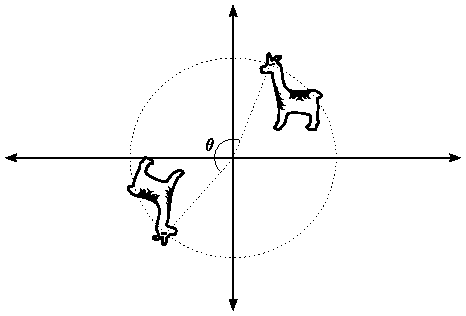
\includegraphics{rotIdeaEg.pdf}
\end{image}
\begin{warning} 
Positive angles denote a counterclockwise rotation. Negative angles
denote a clockwise rotation.
\end{warning}

Looking back on trigonometry, there were some angles that kept on
coming up. Some of these were $90^\circ$, $60^\circ$, and $45^\circ$.
We'll focus on these angles too.
\begin{align*}
\mat{R}_{90} &=
\begin{bmatrix}
0 & -1 & 0\\
1 & 0 & 0\\
0 & 0 & 1
\end{bmatrix}\\
\mat{R}_{60} &=
\begin{bmatrix}
\frac{1}{2} & \frac{-\sqrt{3}}{2} & 0\\
\frac{\sqrt{3}}{2} & \frac{1}{2} & 0\\
0 & 0 & 1
\end{bmatrix}\\
\mat{R}_{45} &=
\begin{bmatrix}
\frac{1}{\sqrt{2}} & \frac{-1}{\sqrt{2}} & 0\\
\frac{1}{\sqrt{2}} & \frac{1}{\sqrt{2}} & 0\\
0 & 0 & 1
\end{bmatrix}
\end{align*}


\begin{example} 
Consider the point $\vec{p} = (4,-2)$. Use a matrix to rotate
$\vec{p}$ $60^\circ$ about the origin.
\begin{image}
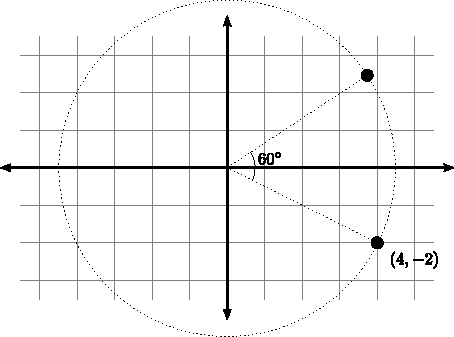
\includegraphics{rotEg1.pdf}
\end{image}
\begin{explanation}
Here is how you do it:
\begin{align*}
\mat{R}_{60} \vec{p} &= 
\begin{bmatrix}
\frac{1}{2} & \frac{-\sqrt{3}}{2} & 0\\
\frac{\sqrt{3}}{2} & \frac{1}{2} & 0\\
0 & 0 & 1
\end{bmatrix}
\begin{bmatrix}
4 \\
-2 \\
1
\end{bmatrix}\\
&=
\begin{bmatrix}
\answer[given]{2+\sqrt{3}}\\
\answer[given]{2\sqrt{3}-1} \\
\answer[given]{1}
\end{bmatrix}
\end{align*}
Hence, we end up with the point $\left(\answer[given]{2+\sqrt{3}},\answer[given]{2\sqrt{3}-1}\right)$.
\end{explanation}
\end{example}


\begin{question}
  Do the numbers in the matrices above look familiar? If so, why?
  \begin{prompt}
    \begin{multipleChoice}
      \choice[correct]{I've thought about this.}
      \choice{I've not thought about this.}
    \end{multipleChoice}
    \begin{idea}
    Hmmm. I think I've seen the numbers that appear in $\mat{R}_{90}$,
    $\mat{R}_{60}$, and $\mat{R}_{45}$ appear in the \link[unit
      circle]{https://en.wikipedia.org/wiki/Unit_circle}! So this
    kinda makes sense!
    \end{idea}
  \end{prompt}
\end{question}


\begin{question}
  How do you rotate a point $180$ degrees?
  \begin{prompt}
    You just apply the matrix
    \begin{validator}[a*t==180]
      $\mat{R}_{\answer[format=integer,id=a]{0}}$
      $\answer[format=integer,id=t]{0}$ times.
    \end{validator}
  \end{prompt}
\end{question}



\begin{question} 
  Can you demonstrate with algebra why $\mat{R}_{60}$ is an isometry?

  \begin{prompt}
    To start we need two points, say $\vec{a} = (a,b)$ and $\vec{p} =
    (p,q)$. Now compute the distance between these two points using
    the distance formula:
    \[
    d(\vec{a},\vec{p}) = \answer{\sqrt{(a-p)^2 + (b-q)^2}}
    \]
    Now we will rotate these two points $60^\circ$  using
    $\mat{R}_{60}$ and show that the distance between the rotated
    points is the same distance found above. Write with me:
    \[
    \mat{R}_{60} \vec{a} =
    \begin{bmatrix}
      \answer{a/2-b\sqrt{3}/2}\\
      \answer{a\sqrt{3}/2+b/2}
    \end{bmatrix}
    \]
    and
    \[
    \mat{R}_{60} \vec{p} =
    \begin{bmatrix}
      \answer{p/2-q\sqrt{3}/2}\\
      \answer{p\sqrt{3}/2+q/2}
    \end{bmatrix}
    \]
    Now, compute the distance between $\mat{R}_{60} \vec{a}$ and
    $\mat{R}_{60} \vec{p}$:
    \[
    d(\mat{R}_{60} \vec{a}, \mat{R}_{60} \vec{p}) =
    \answer{\sqrt{(a-p)^2 + (b-q)^2}}.
    \]
    Since the distances found \wordChoice{\choice{are
        different}\choice[correct]{are the same}}, we see that $\mat{R}_{60}$ is
    an isometry.
  \end{prompt}
\end{question}


\end{document}
